\documentclass[12pt]{article}

\usepackage[a4paper,margin=1in]{geometry}
\usepackage{amsmath,amssymb}
\usepackage{newtxtext,newtxmath} % Times-style font
\usepackage{fancyhdr}
\usepackage{listings}
\usepackage{graphicx}
\usepackage{float}
\usepackage{algorithm}
\usepackage{algpseudocode}

\setlength{\textfloatsep}{10pt}
\setlength{\floatsep}{10pt}

\setlength{\parindent}{0pt}
\setlength{\parskip}{5pt}

% Keep entire document at 12 pt
\AtBeginDocument{
    \fontsize{12pt}{14pt}\selectfont
}

\lstdefinestyle{code}{
    language=Python,
    basicstyle=\ttfamily\fontsize{10pt}{12pt}\selectfont,
    breaklines=true,
    breakatwhitespace=false,
    frame=single,
    numbers=left,
    numberstyle=\tiny\color{gray},
    keywordstyle=\color{blue},
    commentstyle=\color{gray},
    stringstyle=\color{green!50!black},
    columns=fullflexible,
    keepspaces=true,
    showstringspaces=false
}

\lstdefinestyle{output}{
    basicstyle=\ttfamily\fontsize{10pt}{12pt}\selectfont,
    breaklines=true,
    breakatwhitespace=false,
    frame=single,
    numbers=none,
    backgroundcolor=\color{gray!4},
    columns=fullflexible,
    keepspaces=true,
    showstringspaces=false
}

% ------------------------------------------------
% Header
% ------------------------------------------------

\pagestyle{fancy}
\fancyhf{}

\fancyhead[L]{Name: Kishan Sahu{\hspace{4cm}}}
\fancyhead[R]{Enrollment No.: P26DS017{\hspace{3.5cm}}}

\renewcommand{\headrulewidth}{0.4pt}
\setlength{\headheight}{15pt}

\begin{document}

% ------------------------------------------------
% TITLE
% ------------------------------------------------

\begin{center}
\textbf{Computer Science and Engineering Department, SVNIT, Surat}\\
\textbf{M.Tech. I -- Semester I}\\
\textbf{Design and Analysis of Algorithm (CSDS103)}\\
\textbf{Lab Assignment 3}\\
\textbf{Dynamic Programming}
\end{center}

\vspace{0.3cm}

% =========================================================================
% PROBLEM 1
% =========================================================================

\textbf{Problem Statement: 1}

Problem -- Coin Change

\vspace{0.2cm}

\textbf{1. Dynamic Programming Formulation:}
\begin{itemize}
    \item \textbf{Subproblem/State Definition:} Let $DP[a]$ denote the minimum number of coins required to form a target amount $a$, where $0 \le a \le A$.
    \item \textbf{Base Cases:}
    \begin{align*}
        DP[0] &= 0 \quad (\text{0 coins are needed to make an amount of 0}) \\
        DP[a] &= \infty \quad \text{for all } a > 0 \quad (\text{initialized to infinity})
    \end{align*}
    \item \textbf{State Transition (Recurrence Relation):}
    \begin{equation*}
        DP[a] = 1 + \min_{\substack{c \in \text{coins} \\ c \le a}} DP[a - c]
    \end{equation*}
    If $DP[A] = \infty$, then the target amount cannot be formed using the given denominations.
\end{itemize}

\vspace{0.2cm}

\begin{algorithm}[H]
\caption{CoinChangeDP}
\begin{algorithmic}[1]
\State \textbf{ALGORITHM} CoinChangeDP($coins, amount$):
    \State $dp \gets$ Array of size $(amount + 1)$ initialized to $\infty$
    \State $parent \gets$ Array of size $(amount + 1)$ initialized to $-1$
    \State $dp[0] \gets 0$

    \For{$a \gets 1$ \textbf{TO} $amount$}
        \For{\textbf{EACH} $c$ \textbf{IN} $coins$}
            \If{$c \le a$ \textbf{AND} $dp[a - c] + 1 < dp[a]$}
                \State $dp[a] \gets dp[a - c] + 1$
                \State $parent[a] \gets c$
            \EndIf
        \EndFor
    \EndFor

    \If{$dp[amount] = \infty$}
        \State \Return $(-1, [\ ])$
    \EndIf

    \State \textbf{// Reconstruct optimal coin combination}
    \State $combination \gets [\ ]$
    \State $curr \gets amount$
    \While{$curr > 0$}
        \State $c \gets parent[curr]$
        \State Append $c$ to $combination$
        \State $curr \gets curr - c$
    \EndWhile

    \State \Return $(dp[amount], combination)$
\end{algorithmic}
\end{algorithm}

\newpage
\textbf{Code:}

\begin{lstlisting}[style=code]
def coin_change_dp(coins, amount):
    """Bottom-up Dynamic Programming with coin combination reconstruction."""
    dp = [0] + [float('inf')] * amount
    parent = [-1] * (amount + 1)

    for a in range(1, amount + 1):
        for c in coins:
            if c <= a and dp[a - c] + 1 < dp[a]:
                dp[a] = dp[a - c] + 1
                parent[a] = c

    if dp[amount] == float('inf'):
        return -1, []

    # Reconstruct optimal combination
    combination, curr = [], amount
    while curr > 0:
        c = parent[curr]
        combination.append(c)
        curr -= c

    return dp[amount], combination


def coin_change_rec(coins, amount):
    """Naive recursive approach without memoization."""
    if amount == 0:
        return 0
    min_coins = float('inf')
    for c in coins:
        if c <= amount:
            res = coin_change_rec(coins, amount - c)
            if res != float('inf'):
                min_coins = min(min_coins, 1 + res)
    return min_coins


def main():
    # PDF Example: coins = {1, 3, 4}, target amount = 6
    coins = [1, 3, 4]
    amount = 6

    min_coins, combo = coin_change_dp(coins, amount)
    print(f"Denominations : {coins}")
    print(f"Target Amount : {amount}")
    print(f"Minimum Coins : {min_coins}")
    print(f"Combination   : {' + '.join(map(str, combo))} = {amount}")

    # Boundary Cases
    print("\n--- Boundary Cases ---")
    print(f"Target 0: min_coins = {coin_change_dp(coins, 0)[0]}, combination = {coin_change_dp(coins, 0)[1]}")
    print(f"Unreachable Target (coins=[2, 4], amount=7): {coin_change_dp([2, 4], 7)}")


if __name__ == "__main__":
    main()
\end{lstlisting}

\textbf{Output:}

\begin{lstlisting}[style=output]
Denominations : [1, 3, 4]
Target Amount : 6
Minimum Coins : 2
Combination   : 3 + 3 = 6

--- Boundary Cases ---
Target 0: min_coins = 0, combination = []
Unreachable Target (coins=[2, 4], amount=7): (-1, [])
\end{lstlisting}

\newpage
\textbf{Complexity Comparison (DP vs. Naive Recursion):}

\begin{table}[H]
\centering
\begin{tabular}{|p{3.2cm}|p{3.2cm}|p{8.0cm}|}
\hline
\textbf{Approach} & \textbf{Time Complexity} & \textbf{Auxiliary Space} \\
\hline
\textbf{Bottom-Up DP} & $\mathcal{O}(n \cdot A)$ & $\mathcal{O}(A)$ (DP and parent tracking tables) \\
\hline
\textbf{Naive Recursive} & $\mathcal{O}(n^A)$ (Exponential) & $\mathcal{O}(A)$ (Maximum recursion call stack depth) \\
\hline
\end{tabular}
\caption{Theoretical complexity comparison for Coin Change ($n = |\text{coins}|$, $A = \text{amount}$).}
\end{table}

\textbf{Empirical Execution Time Experimentation:}

\begin{figure}[H]
\centering
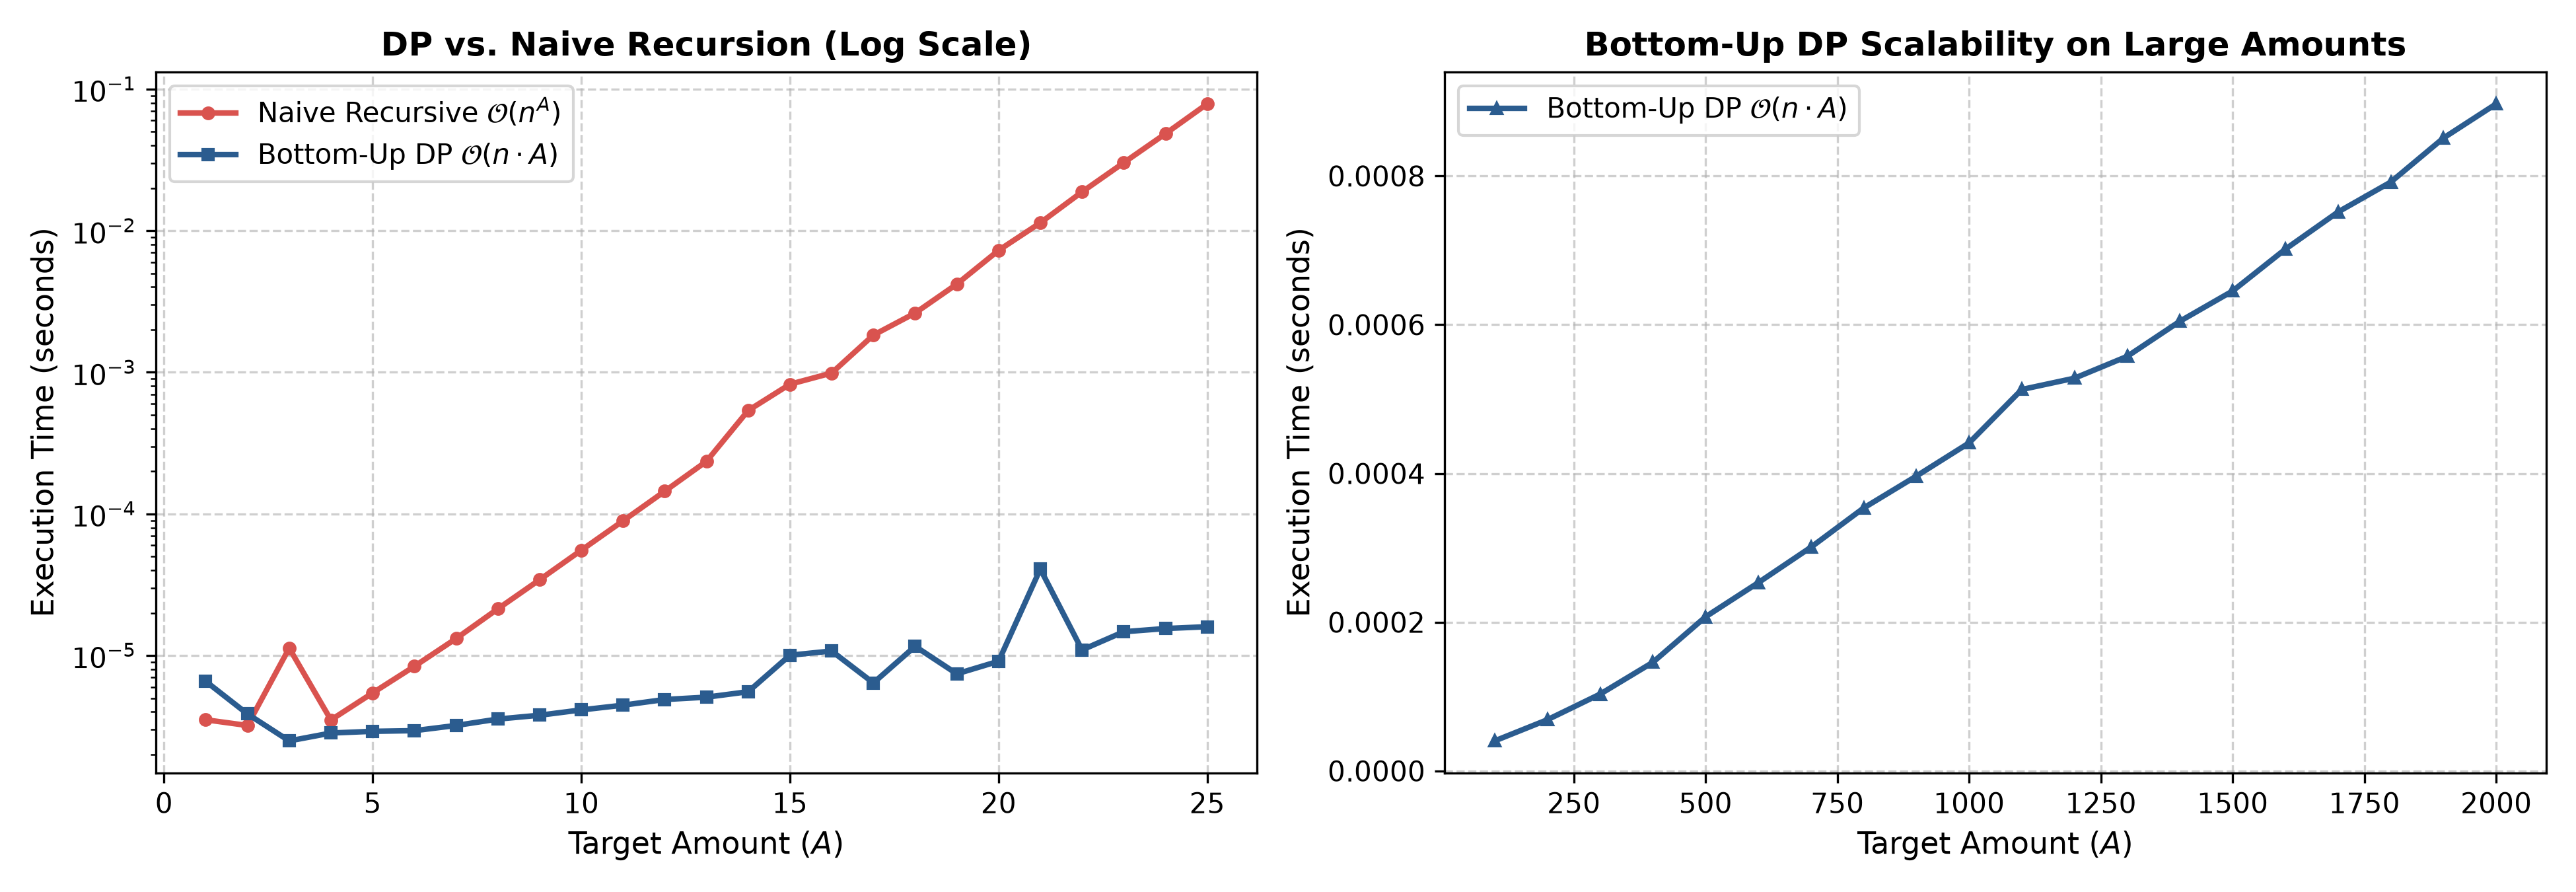
\includegraphics[width=0.92\textwidth]{plot_coin_change.png}
\caption{Execution time comparison: (Left) Log-scale execution time comparing DP $\mathcal{O}(n \cdot A)$ vs. Naive Recursion $\mathcal{O}(n^A)$ for $A \in [1, 25]$; (Right) Linear scalability of Bottom-Up DP for large amounts up to $A = 2000$.}
\end{figure}

\textbf{Analysis:}

\textbf{1. Greedy Strategy Evaluation:}
A greedy strategy selects the largest available denomination $c \le \text{remaining amount}$ at every step. While this produces the optimal minimum number of coins for canonical currency systems (e.g., standard denominations), it does \textbf{not} always guarantee an optimal solution for arbitrary coin systems.

\textbf{2. Counterexample (from PDF):}
Consider coin denominations $\{1, 3, 4\}$ and target amount $6$:
\begin{itemize}
    \item \textbf{Greedy Strategy:}
    \begin{enumerate}
        \item Step 1: Chooses denomination $4$ (Remaining amount: $6 - 4 = 2$).
        \item Step 2: Chooses denomination $1$ (Remaining amount: $2 - 1 = 1$).
        \item Step 3: Chooses denomination $1$ (Remaining amount: $1 - 1 = 0$).
        \item \textbf{Total coins selected by Greedy:} $3$ coins ($4 + 1 + 1 = 6$).
    \end{enumerate}
    \item \textbf{Dynamic Programming (Optimal):}
    \begin{enumerate}
        \item Evaluates subproblems $DP[6 - 3] + 1 = DP[3] + 1 = 1 + 1 = 2$.
        \item \textbf{Total coins selected by DP:} $2$ coins ($3 + 3 = 6$).
    \end{enumerate}
\end{itemize}

\textbf{3. Why Dynamic Programming Succeeds where Greedy Fails:}
The greedy approach makes a short-sighted local optimum (picking $4$) without considering how that choice restricts future decisions. In contrast, Dynamic Programming examines all valid coin transitions $DP[a - c] + 1$ across every subproblem amount $a$. By utilizing \textbf{optimal substructure} and memoizing optimal subproblem solutions, DP guarantees finding the global minimum.

\newpage

% =========================================================================
% PROBLEM 2
% =========================================================================

\textbf{Problem Statement: 2}

Problem -- Employee Training Planning

\vspace{0.2cm}

\textbf{1. Dynamic Programming Formulation (0/1 Knapsack):}
\begin{itemize}
    \item \textbf{Problem Formulation:} Given $n$ training modules with costs $c_i$ and benefits $b_i$, and a maximum training budget $B$, select a subset of modules to maximize total benefit such that total cost $\le B$. Each module can be selected at most once.
    \item \textbf{State Definition:} Let $DP[i][w]$ denote the \textbf{maximum achievable benefit} considering a subset of the first $i$ modules under budget constraint $w$, where $0 \le i \le n$ and $0 \le w \le B$.
    \item \textbf{Base Cases:}
    \begin{align*}
        DP[0][w] &= 0 \quad \text{for all } 0 \le w \le B \quad (\text{0 benefit if no modules are chosen}) \\
        DP[i][0] &= 0 \quad \text{for all } 0 \le i \le n \quad (\text{0 benefit if budget is 0})
    \end{align*}
    \item \textbf{State Transition (Recurrence Relation):}
    \begin{equation*}
        DP[i][w] = \begin{cases}
            DP[i-1][w] & \text{if } c_i > w \\
            \max\Big(DP[i-1][w], \; DP[i-1][w - c_i] + b_i\Big) & \text{if } c_i \le w
        \end{cases}
    \end{equation*}
\end{itemize}

\vspace{0.2cm}

\begin{algorithm}[H]
\caption{EmployeeTrainingDP}
\begin{algorithmic}[1]
\State \textbf{ALGORITHM} EmployeeTrainingDP($modules, budget$):
    \State $n \gets Length(modules)$
    \State $dp \gets$ 2D Array of size $(n + 1) \times (budget + 1)$ initialized to $0$

    \For{$i \gets 1$ \textbf{TO} $n$}
        \State $(name_i, c_i, b_i) \gets modules[i - 1]$
        \For{$w \gets 0$ \textbf{TO} $budget$}
            \If{$c_i \le w$}
                \State $dp[i][w] \gets \max(dp[i - 1][w], \; dp[i - 1][w - c_i] + b_i)$
            \Else
                \State $dp[i][w] \gets dp[i - 1][w]$
            \EndIf
        \EndFor
    \EndFor

    \State \textbf{// Reconstruct optimal module subset}
    \State $selected \gets [\ ]$
    \State $w \gets budget$
    \For{$i \gets n$ \textbf{DOWNTO} $1$}
        \If{$dp[i][w] \neq dp[i - 1][w]$}
            \State $(name_i, c_i, b_i) \gets modules[i - 1]$
            \State Append $name_i$ to $selected$
            \State $w \gets w - c_i$
        \EndIf
    \EndFor

    \State Reverse($selected$)
    \State \Return $(dp[n][budget], selected)$
\end{algorithmic}
\end{algorithm}

\newpage
\textbf{Code:}

\begin{lstlisting}[style=code]
def employee_training_01_dp(modules, budget):
    """
    Bottom-up 0/1 Dynamic Programming for Employee Training Planning.
    modules: list of tuples (name, cost, benefit)
    budget: maximum training budget B
    """
    n = len(modules)
    dp = [[0] * (budget + 1) for _ in range(n + 1)]

    for i in range(1, n + 1):
        name, cost, benefit = modules[i - 1]
        for w in range(budget + 1):
            if cost <= w:
                dp[i][w] = max(dp[i - 1][w], dp[i - 1][w - cost] + benefit)
            else:
                dp[i][w] = dp[i - 1][w]

    # Reconstruct selected modules
    selected_modules = []
    w = budget
    total_cost = 0
    for i in range(n, 0, -1):
        if dp[i][w] != dp[i - 1][w]:
            name, cost, benefit = modules[i - 1]
            selected_modules.append(name)
            total_cost += cost
            w -= cost

    selected_modules.reverse()
    return dp[n][budget], total_cost, selected_modules


def main():
    # PDF Module Data
    modules = [
        ("M1", 4, 7),
        ("M2", 6, 10),
        ("M3", 5, 8),
        ("M4", 3, 5)
    ]
    budget = 10

    max_benefit, total_cost, selected = employee_training_01_dp(modules, budget)

    print("=== PDF Example Solution (Budget B = 10) ===")
    print(f"Available Modules : {modules}")
    print(f"Maximum Benefit   : {max_benefit}")
    print(f"Total Cost        : {total_cost} / {budget}")
    print(f"Selected Modules  : {selected}")

    # Boundary Cases
    print("\n--- Boundary Cases ---")
    print(f"Budget 0 : {employee_training_01_dp(modules, 0)}")
    print(f"Budget 2 (Below minimum module cost): {employee_training_01_dp(modules, 2)}")


if __name__ == "__main__":
    main()
\end{lstlisting}

\textbf{Output:}

\begin{lstlisting}[style=output]
=== PDF Example Solution (Budget B = 10) ===
Available Modules : [('M1', 4, 7), ('M2', 6, 10), ('M3', 5, 8), ('M4', 3, 5)]
Maximum Benefit   : 17
Total Cost        : 10 / 10
Selected Modules  : ['M1', 'M2']

--- Boundary Cases ---
Budget 0 : (0, 0, [])
Budget 2 (Below minimum module cost): (0, 0, [])
\end{lstlisting}

\newpage
\textbf{Complexity Analysis:}

\begin{table}[H]
\centering
\begin{tabular}{|p{3.2cm}|p{3.2cm}|p{8.0cm}|}
\hline
\textbf{Implementation} & \textbf{Time Complexity} & \textbf{Auxiliary Space} \\
\hline
\textbf{2D Bottom-Up DP} & $\mathcal{O}(n \cdot B)$ & $\mathcal{O}(n \cdot B)$ (Table of size $(n+1) \times (B+1)$) \\
\hline
\textbf{1D Space-Optimized} & $\mathcal{O}(n \cdot B)$ & $\mathcal{O}(B)$ (Single 1D array traversed backwards) \\
\hline
\end{tabular}
\caption{Complexity breakdown for Employee Training Planning ($n = \text{number of modules}$, $B = \text{budget}$).}
\end{table}

\textbf{Empirical Execution Time Experimentation:}

\begin{figure}[H]
\centering
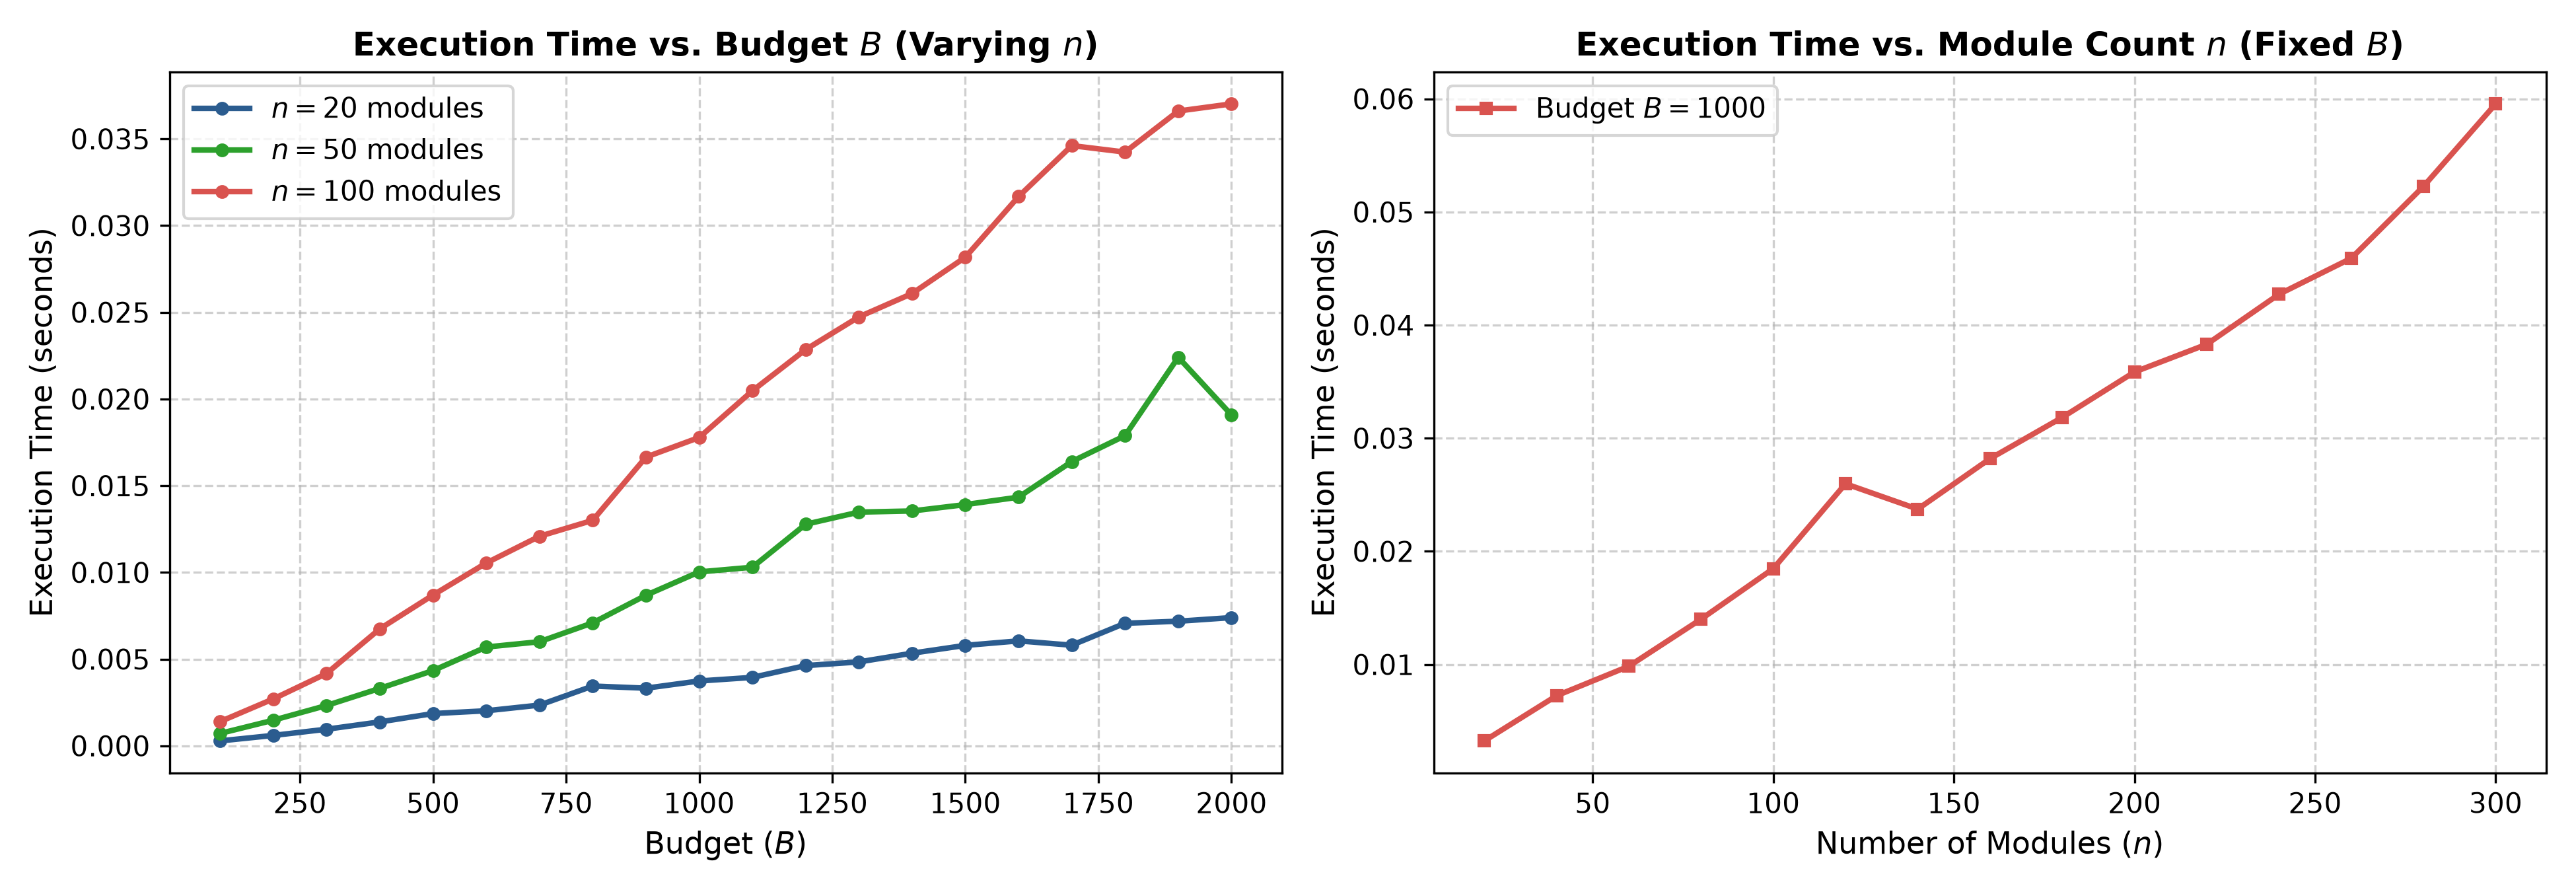
\includegraphics[width=0.92\textwidth]{plot_employee_training.png}
\caption{Empirical execution time analysis: (Left) Linear scaling with budget $B$ across different module counts $n \in \{20, 50, 100\}$; (Right) Linear scaling with module count $n$ for fixed budget $B = 1000$.}
\end{figure}

\textbf{Analysis:}

\textbf{1. Problem Formulation under Module Repetition (Unbounded Knapsack):}
When training modules may be selected \textbf{more than once}, the constraint transitions from a 0/1 decision to an \textbf{Unbounded Knapsack} problem.

\textbf{2. Mathematical Formulation \& Recurrence Changes:}
\begin{itemize}
    \item \textbf{0/1 Constraint:} Once module $i$ is chosen, the remaining budget must be filled using only the remaining $i-1$ modules:
    \begin{equation*}
        DP[i][w] = \max\Big(DP[i-1][w], \; DP[i-1][w - c_i] + b_i\Big)
    \end{equation*}
    \item \textbf{Unbounded Modification:} Module $i$ can be repeatedly selected from the current state $w - c_i$:
    \begin{equation*}
        DP[w] = \max_{\substack{1 \le i \le n \\ c_i \le w}} \Big(DP[w - c_i] + b_i\Big), \quad \text{with } DP[0] = 0
    \end{equation*}
\end{itemize}

\textbf{3. Effect on Selection Behavior \& Complexity:}
\begin{itemize}
    \item \textbf{Selection Behavior:} The algorithm can repeatedly exploit the module with the highest benefit-to-cost efficiency ratio $\frac{b_i}{c_i}$.
    \begin{itemize}
        \item For the PDF modules: $M_1 (7/4 = 1.75)$, $M_2 (10/6 \approx 1.67)$, $M_3 (8/5 = 1.60)$, $M_4 (5/3 \approx 1.67)$.
        \item For budget $B = 12$, the 0/1 optimal solution selects $M_1 + M_3 + M_4$ with total Benefit = \textbf{20}.
        \item In contrast, the Unbounded solution selects $M_1 \times 3$ with total Benefit = \textbf{21} ($3 \times 7$), achieving strictly higher benefit.
    \end{itemize}
    \item \textbf{Space Complexity:} Reduces from $\mathcal{O}(n \cdot B)$ in 2D to $\mathcal{O}(B)$ in 1D array formulation.
    \item \textbf{Time Complexity:} Remains $\mathcal{O}(n \cdot B)$, requiring $n$ transitions for each budget step $1 \dots B$.
\end{itemize}

\end{document}
